\section{Large worlds of mathematical structures}
\subsection{Monoids and Homomorphisms}
Suppose some function $f: \mathbb{N} \rightarrow \mathbb{Z}$ and $f(n)=n$. This function
$f$ respects addition in the following sense.
\begin{align*}
    f(m+n) = f(m) + f(n)
\end{align*}
We can add $m+n$ first and then map it via $f$, or we can first map $m, n$ via
$f$, and then add them.

\begin{ttta}
Another possible function $f: \mathbb{N} \rightarrow \mathbb{Z}$ is given by
$f(n) = 2n$. See if you can check that this also satisfies the above condition
$f(m+n) = f(m) + f(n)$.
\begin{align*}
    f(m+n) =& f(m) + f(n)\\
    2(m+n) =& 2(m) + 2(n)\\
    2(m+n) =& 2(m+n)\\
    m+n =& m+n
\end{align*}
Thus we have shown that $f$ respects addition.
\end{ttta}

\begin{ttta}
Show that this function
\[
f=\set{(0, 0), (1, 1), (2, -1), (3, 2), (4, -2), (5, 3), (6, -3), \dots}
\]
does not respect addition.
\begin{align*}
    f(1+3) =& f(1) + f(3)\\
    f(4) =& f(1) + f(3)\\
    -2 =& 1 + 2\\
    -2 \neq& 3
\end{align*}
\end{ttta}

\begin{ttta}
Mapping into the integers is special because it turns out that respecting
addition forces a function to respect the identity. Prove it.
\end{ttta}
\begin{proofitem}
\item To respect addition a function $f$ must satisfy the following equation $f(m+n) =
f(m)+f(n)$.  Let us suppose that $f$ does respect addition and show that it
implies that $f$ also respects the identity.
\begin{align*}
    f(0+n) =& f(0) + f(n)\\
    f(n) =& f(0) + f(n)\\
    f(0) =& 0
\end{align*}
\end{proofitem}
\begin{definition}
Let $A$ and $B$ be monoids, and write the identity as $1$ and the
binary operation as $\circ$ in each case. Then a monoid homomorphism from A to
B is a function $f:A\rightarrow B$ on the underlying sets, such that
\begin{align*}
    \forall x, y \in A, f(x \circ y) &= f(x) \circ f(y)&&f\text{ respects }\circ\\
    f(1)&=1&&f\text{ respects identity}
\end{align*}
\end{definition}

\stepcounter{tttacounter}
\begin{ttta}
What do we need to check to show that monoids and their homomorphisms form a
category?
\end{ttta}
\begin{proofitem}
\item Let $M$ be the set of monoids, $M_A, M_B, M_C, \ldots, \in M$.
\item Let $\mathcal{C}_\text{mon}$ be a category where each object is a monoid
    $A\in M$, and each arrow $\times$ is a mapping $A,B \in M, \times:
    A\rightarrow B$.
\item Let $f, g$ be composable functions, ie they are arrows between objects.
\item Let $\circ$ be a binary composition operation on arrows.
\item Let $\ast$ be a binary composition operation on monoidal elements.
\item To show that monoids and their homomorphisms form a cateogry we must show
    the properties of unitality and associativity.
\setcounter{equation}{0}
\begin{align}
    (g\circ f)(x\ast y) &= g(f(x\ast y)) && \text{def. of }\circ\\
    &= g(f(x) \ast f(y)) && f\text{ respects }\ast\\
    &= g(f(x)) \ast g(f(y)) && g\text{ respects }\ast\\
    &= (g\circ f)(x) \ast (g\circ f)(y) && \text{def. of }\circ\\
    (g\circ f)(1)&= g(f(1)) && \text{def. of }\circ\\
    &= g(1) && f \text{ respects }1\\
    &= 1 && g \text{ respects }1
\end{align}
\end{proofitem}
\begin{figure}[H]
\documentclass[border=0.2cm]{standalone}
\usepackage{tikz}
\usepackage{titlesec}
\usepackage{float}
\usepackage{standalone}
\usepackage{tikzit}
\usetikzlibrary{automata, arrows.meta, positioning}
\usetikzlibrary{arrows.meta, positioning}
\input{figures/sample-02.tikzstyles}

\begin{document}
\begin{tikzpicture}[scale=1.0]
	\begin{pgfonlayer}{nodelayer}
		\node [style=object] (0) at (0, 0) {$M_A$};
		\node [style=object] (1) at (4, 0) {$M_B$};
		\node [style=object] (2) at (8, 0) {$M_C$};
	\end{pgfonlayer}
	\begin{pgfonlayer}{edgelayer}
		\path [-stealth, thick]
		(0) edge node[above] {$f$}   (1)
		(1) edge node[above] {$g$}   (2)
		(0) edge [out=210, in=240, looseness=8, below]  node {$x$}(0)
		(0) edge [out=330, in=300, looseness=8, below]  node {$y$}(0)
		(0) edge [loop above] node[above] {$x\ast y$}(0)
		(1) edge [out=210, in=240, looseness=8, below]  node {$x$}(1)
		(1) edge [out=330, in=300, looseness=8, below]  node {$y$}(1)
		(1) edge [loop above] node[above] {$f(x\ast y)$}(1)
		(2) edge [out=210, in=240, looseness=8, below]  node {$x$}(2)
		(2) edge [out=330, in=300, looseness=8, below]  node {$y$}(2)
		(2) edge [loop above] node[above] {$(g\circ f)(x\ast y)$}(2) ;
	\end{pgfonlayer}
\end{tikzpicture}
\end{document}

\caption{Monoid Category $\mathbf{Monoid}$}
\end{figure}
\subsection{Groups}
\begin{ttta}
Define group homomorphism as a function respecting the group structure. When
dealing with groups, it is redundant to ask for the identity to be preserved.
It’s also redundant to ask for the inverses to be preserved. Prove this.
\end{ttta}
\begin{proofitem}
\item The properties needed for a group are identity, inverse, and
    associativity. We can show that if there exists a function $f$ which is a
    group homomorphism, then we get inverse and identity for freebeez.
\item Suppose $f: G \rightarrow H$ is a homomorphism between groups $G$ and $H$. Then:
\begin{align*}
    f(x\ast x^{-1}) &= f(1_G)\\
    f(x)\ast f(x^{-1}) &= 1_H
\end{align*}
\item Therefore $f(x^{-1})$ is indeed the inverse of $f(x)$ and inverse is
    preserved.
\begin{align*}
    f(x\ast 1_G) &= f(x)\\
    f(x)\ast f(1_G) &= f(x)\\
    f(x^{-1})\ast f(x)\ast 1_H &= f(x^{-1})\ast f(x)\\
    1_H &= f(x^{-1}\ast x)\\
    1_H &= f(1_G)
\end{align*}
\item Therefore identity is preserved.
\end{proofitem}

\begin{ttta}
Do we have to check anything else to show that groups and group homomorphisms form a category?
\end{ttta}
Because groups are monoids with an extra property, there is nothing to check
because monoids already form a cateogry. In other words, the monoidal nature of
a group is sufficient to show unitality and associativity for a category created
from some set that is also a group.

\subsection{Posets}
\begin{ttta}
Create a definition of an order-preserving function for posets in general by
analogy with the structure-preserving maps we've seen already.
\end{ttta}
\begin{proofitem}
\item Let $f:P\rightarrow Q$ be some function between two posets $P$ and $Q$.
    Because $P$ and $Q$ are posets, we know that individually they both have the
    properties reflexivity, transitivity, and antisymmetry. For $f$ to be order
    preserving, the only condition on $f$ is
\begin{align*}
    x\geq_P y \implies f(x)\geq_Q f(y)
\end{align*}
\end{proofitem}

\begin{ttta}
Do we have to check anything to show that we have a category of posets and order-preserving functions?
\end{ttta}
\begin{proofitem}
    \item To check that we have a category, we must assure unitality and
        associativity are preserved.
\end{proofitem}
\begin{align*}
    x \geq y &\implies f(x) \geq f(y) \\
             &\implies g(f(x) \geq g(f(y)) \\
             &\implies (g\circ f)(x) \geq (g\circ f)(y) \\
\end{align*}
\begin{figure}[H]
    \begin{center}
\documentclass[border=0.2cm]{standalone}
\usepackage{tikz}
\usepackage{titlesec}
\usepackage{float}
\usepackage{standalone}
\usepackage{tikzit}
\usetikzlibrary{automata, arrows.meta, positioning}
\usetikzlibrary{arrows.meta, positioning}
\input{sample-02.tikzstyles}

\begin{document}
\begin{tikzpicture}
	\begin{pgfonlayer}{nodelayer}
		\node [style=object] (0) at (0, 0) {$P_A$};
		\node [style=object] (1) at (4.5, 0) {$P_B$};
		\node [style=object] (2) at (9, 0) {$P_C$};
	\end{pgfonlayer}
	\begin{pgfonlayer}{edgelayer}
        \path [-stealth, thick]
        (0) edge node[above] {$f$}   (1)
        (1) edge node[above] {$g$}   (2)
        (0) edge [out=30, in=60, looseness=8, below]  node[above] {$1$}(0)
        (0) edge [out=120, in=150, looseness=8, below] node[above] {$x\ast y$}(0)
        (0) edge [out=210, in=240, looseness=8, below]  node[below] {$x$}(0)
        (0) edge [out=300, in=330, looseness=8, below]  node[below] {$y$}(0)
        (1) edge [out=30, in=60, looseness=8, below]  node[above] {$f(1)$}(1)
        (1) edge [out=120, in=150, looseness=8, below] node[above] {$f(x\ast y$)}(1)
        (1) edge [out=210, in=240, looseness=8, below]  node[below] {$f(x)$}(1)
        (1) edge [out=300, in=330, looseness=8, below]  node[below] {$f(y)$}(1)
        (2) edge [out=30, in=60, looseness=8, below]  node[above, xshift=1cm] {$(g\circ f)(1)$}(2)
        (2) edge [out=120, in=150, looseness=8, below] node[xshift=-0.4cm,above] {$(g\circ f)(x\ast y$)}(2)
        (2) edge [out=210, in=240, looseness=8, below]  node[xshift=-0.5cm, below] {$(g\circ f)(x)$}(2)
        (2) edge [out=300, in=330, looseness=8, below]  node[xshift=0.5cm, below] {$(g\circ f)(y)$}(2)
        ;
	\end{pgfonlayer}
\end{tikzpicture}
\end{document}

\end{center}
\caption{Poset Category $\mathbf{Poset}$}
\end{figure}

\begin{ttta}
Think again about the poset of factors of 42.
Observe that $6 < 7$ but 6 is higher than 7 in this diagram. What two orderings
are we considering on the same set of numbers here, and what map is it that is
not order-preserving?
\end{ttta}
\begin{figure}[H]
    \begin{center}
        \documentclass[border=0.2cm]{standalone}
\usepackage{tikz}
\usepackage{titlesec}
\usepackage{float}
\usepackage{standalone}
\usepackage{tikzit}
\usetikzlibrary{automata, arrows.meta, positioning}
\usetikzlibrary{arrows.meta, positioning}
\input{sample-02.tikzstyles}

\begin{document}
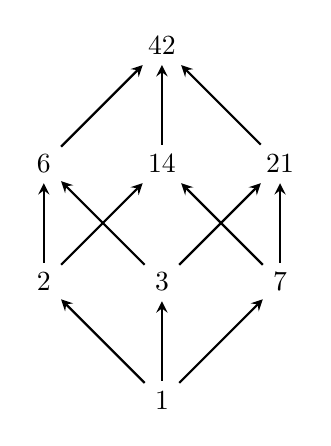
\begin{tikzpicture}[->, >=stealth, thick]
\node (1) at (3,0) {$1$};
\node (2) at (1.5,1.5) {$2$};
\node (3) at (3,1.5) {$3$};
\node (5) at (4.5,1.5) {$7$};
\node (6) at (1.5,3) {$6$};
\node (10) at (3,3) {$14$};
\node (15) at (4.5,3) {$21$};
\node (30) at (3,4.5) {$42$};
\draw (1) -- (2);
\draw (1) -- (3);
\draw (1) -- (5);
\draw (2) -- (6);
\draw (2) -- (10);
\draw (3) -- (6);
\draw (3) -- (15);
\draw (5) -- (10);
\draw (5) -- (15);
\draw (6) -- (30);
\draw (10) -- (30);
\draw (15) -- (30);
\end{tikzpicture}
\end{document}

    \end{center}
    \caption{42-factor lattice}
\end{figure}
\begin{proofitem}
\item Let $S=\set{1,2, 3, 6, 7, 14, 21, 42}\subset \mathbb{N}$.
\item One order is $\geq$ as defined on $\mathbb{N}$.
    The other order is divides $\mid$, as in $a\mid b$---for example $6\mid 12$.
    Both orders are reflexive, anti-symmetric, and transitive, as required by
    definition.
\item Let us consider the map $f:\mathbb{N}\rightarrow\mathbb{N}$, where $f=+1$.
    For the ordering $\geq$, $f$ preserves ordering.
\begin{align*}
    f(x \geq y) =& f(x) \geq f(y)\\
        =& x+1 \geq y+1\\
        =& x \geq y
\end{align*}
Now we will show that $f$ does not preserve ordering on $\mid$ by
counter-example.
\begin{align*}
    f(x \mid y) =& f(x) \mid f(y)&&\text{Let }x=7, y=14\\
    f(7 \mid 14) =& f(7) \mid f(14)\\
     \neq& 8 \mid 15
\end{align*}
Thus we have shown that $\mid$ does not preserve ordering.
\end{proofitem}

\subsection{Categories}
\begin{ttta}
Think of a sensible starting point for a definition of a morphism of
categories $F: \mathbb{C} \longrightarrow \mathbb{D}$. It should map objects to
objects and arrows to arrows, but if we start with an arrow $x \xrightarrow{f}
y\in\mathbb{C}$ what should the source and target of $F(f)$ be in
$\mathbb{D}$?
\end{ttta}
\begin{proofitem}
    \item
    \begin{align*}
        f\in \mathbb{C}&: x \rightarrow y\\
        F(f)\in \mathbb{D}&: F(x) \rightarrow F(y)
    \end{align*}
\end{proofitem}

\begin{ttta}
Come up with the definition of a morphism between categories, starting
with the action of $F$ on objects and arrows. Then proceeding by making
sure it is structure-preserving. To do this, you need to be clear what the
structure of a category is: identities and composition. Once you've done this,
can you check that this gives us a category of small categories and all
morphisms between them.
\end{ttta}
